\documentclass{article}

\newcommand{\bra}[1]{\left(#1\right)}
\usepackage[activate={true,nocompatibility},final,tracking=true,kerning=true,spacing=true,factor=1100,stretch=10,shrink=10]{microtype}
\microtypecontext{spacing=nonfrench}
\usepackage{tikz}
\usepackage{tikz-cd}
\usepackage{mathpazo}
\usepackage{amsmath,amsthm,amssymb}
\usepackage{subcaption}
\usepackage{enumerate}
\usepackage{tabularx}
\usetikzlibrary{shapes}
\usetikzlibrary{positioning}
% Set up the images/graphics package
\usepackage{graphicx,float}
\setkeys{Gin}{width=\linewidth,totalheight=\textheight,keepaspectratio}
\graphicspath{{.}}


% Small sections of multiple columns
\usepackage{multicol}
\usepackage[margin=1.6in]{geometry}

%--------Theorem Environments--------
%theoremstyle{plain} --- default
\newtheorem{thm}{Theorem}
\newtheorem{cor}[thm]{Corollary}
\newtheorem{prop}[thm]{Proposition}
\newtheorem{lem}[thm]{Lemma}
\newtheorem{conj}[thm]{Conjecture}
\newtheorem{quest}[thm]{Question}
\newtheorem{claim}{Claim}

\theoremstyle{definition}
\newtheorem{defn}[thm]{Definition}
\newtheorem{defns}[thm]{Definitions}
\newtheorem{con}[thm]{Construction}
\newtheorem{exmp}[thm]{Example}
\newtheorem{jk}[thm]{Joke}
\newtheorem{exmps}[thm]{Examples}
\newtheorem{notn}[thm]{Notation}
\newtheorem{notns}[thm]{Notations}
\newtheorem{addm}[thm]{Addendum}
\newtheorem{exer}[thm]{Exercise}

\theoremstyle{remark}
\newtheorem{rem}[thm]{Remark}
\newtheorem{ans}[thm]{Answer}
\newtheorem{rems}[thm]{Remarks}
\newtheorem{warn}[thm]{Warning}
\newtheorem{sch}[thm]{Scholium}

% MACROS
\newcommand{\Mod}[1]{\ (\text{mod}\ #1)}
\newcommand{\R}{\mathbb{R}}
\newcommand{\N}{\mathbb{N}}
\newcommand{\Q}{\mathbb{Q}}
\newcommand{\F}{\mathbb{F}}
\newcommand{\Z}{\mathbb{Z}}
\newcommand{\mC}{\mathcal{C}}
\newcommand{\mG}{\mathcal{G}}
\newcommand{\mP}{\mathcal{P}}
\newcommand{\one}{\mathbb{1}}
\renewcommand{\P}{\mathbb{P}}
\DeclareMathOperator{\dist}{dist}
\DeclareMathOperator{\aut}{Aut}
\DeclareMathOperator{\gal}{Gal}
\DeclareMathOperator{\orb}{Orb}
\DeclareMathOperator{\stab}{Stab}
\DeclareMathOperator{\inn}{Inn}
\DeclareMathOperator{\spn}{Span}
\DeclareMathOperator{\out}{Out}
\DeclareMathOperator{\im}{Im}
\DeclareMathOperator{\arr}{Arr}
\DeclareMathOperator{\rk}{rk}
\DeclareMathOperator{\rcf}{rcf}
\DeclareMathOperator{\tors}{Tors}
\DeclareMathOperator{\Hom}{Hom}
\DeclareMathOperator{\ann}{Ann}
\DeclareMathOperator{\syl}{Syl}
\newcommand{\norm}[1]{\left\lVert #1 \right\rVert}
\newcommand{\inp}[2]{\left\langle #1, #2 \right\rangle}
\newcommand{\id}{\text{id}}
\newcommand{\gln}{\text{GL}_n}
\newcommand{\op}[1]{#1^{\text{op}}}

\title{Lecture 1 - Categories and Functors\vspace{-10pt}}
\date{\vspace{-30pt}\today\vspace{-20pt}}  % if the \date{} command is left out, the current date will be used
\begin{document}
\maketitle
\begin{abstract} Categories and functors will be introduced as well as lots of examples coming from diverse subfields of mathematics.
\end{abstract}
\setcounter{section}{-1}
\section{Introduction}
This is the first lecture of the Category Theory Student Seminar given at ENS de Lyon. The aim of this course is to teach undergraduate and early graduate students about the basic concepts in category theory. The prerequisites are a basic knowledge of abstract algebra (groups, rings, etc...) and some mathematical maturity. In order to give as many examples as we can, we need to resort to definitions outside of the prerequisites (posets, topological spaces, etc...). They will be omitted in the written notes, but they will be detailed during the lectures.

Before diving into the definitions and examples which almost make up this entire lecture, we discuss a sticky point in our mathematical foundations. Several times in our coverage of category theory, we will use the term \textbf{collection} in order to avoid set theoretical paradoxes. We do not make it more formal because there are many ways to do it (classes, Grothendieck universes, etc.), none of them are really relevant to this course. However, you still need to know why we cannot use sets as is usual in all other courses.

In short, there exist collections of objects that cannot be sets. Famous examples include the class of ordinal numbers which, by the Burali-Forti paradox, cannot be a set and the class of all sets that do not contain themselves which, by the Russel paradox, cannot be a set. In our case, we will need to talk about the collection of all sets and the collection of all groups (among others) and the cannot form sets. For the former, it is easy to see because if $S$ is the set of all sets, then it contains all its subsets and hence $\mP(S) \subseteq S$, this leads to the contradiction $|\mP(S)| \leq |S| < |\mP(S)|$.

\section{Categories}
%TODO: monoides, le voir comme un objet avec des endo fleches pour chaque element. IMPORTANT: fleche et composition. -> Qu'est-ce qu'il se passe quand y a plusieurs objets? -> Intuition pour les catégories, formaliser par la notion de graphe orienté. 
Before giving any definitions, let us start with an example. Let $M$ be a monoid, that is, a set endowed with an associative binary operation $\star$ and a neutral element $e$ (i.e.: a group without inverses). We can represent $M$ with a graph containing a unique point $*$ and for each element $m\in M$ we draw an arrow from $*$ to $*$. Any sequence of arrows (also called path) in this graph corresponds to a sequence of element in $M$. Then, since we can combine these elements using the monoid operation, this path also corresponds to an element of $M$ (i.e. an arrow in the graph). As an example, let $m,n \in M$ be represented in the diagram below, following the arrow $m$ and then the arrow $n$ corresponds to following the arrow $m\star n$. (The point $\ast$ is duplicated to better show the intuition, but there is only one point in the graph.)
\begin{center}
\begin{tikzcd}
\ast \arrow[r, "m"'] \arrow[rr, "n\star m", bend left] & \ast \arrow[r, "n"'] & \ast
\end{tikzcd}
\end{center}
Note that the associativity of $\star$ is essential. Without it, a path $\{m,n,o\}$ could correspond to two different arrows $(m\star n) \star o$ and $m\star (n\star o)$. The notion of category is a suitable generalization of this idea where we allow several points. We first formalize some intuitions with oriented graphs.

\begin{defn}[Oriented graph]
	An \textbf{oriented graph} $G$ consists of a collection of \textbf{nodes/objects} denoted $G_0$ and a collection of \textbf{arrows/morphisms} denoted $G_1$ along with two maps $s,t: G_1 \rightarrow G_0$, so that each arrow $f \in G_1$ has a \textbf{source} $s(f)$ and a \textbf{target} $t(f)$. 
\end{defn}
\begin{defn}[Paths]
	A \textbf{path} in an oriented graph $G$ is a sequence of arrows $(f_1, \dots, f_k)$ that are \textbf{composable} in the sense that $t(f_i) = s(f_{i-1})$ for $i=2,\dots, k$ as seen below. The collection of paths of length $k$ will be denoted $G_k$.
	\begin{figure}[h!]
		\centering
		\begin{tikzcd}
			\bullet \arrow[r, "f_k"] & \bullet \arrow[r, "f_{k-1}"] & \bullet\cdots\bullet \arrow[r, "f_2"] & \bullet \arrow[r, "f_1"] & \bullet
		\end{tikzcd}
		\caption*{Representation of path $(f_1, \dots, f_k)$.}
	\end{figure}
\end{defn}

Observe that the notation indicating the direction of the path does not correspond to the usual notation in graph theory. The motivation for this divergence will come shortly as the composition of arrows in a category is defined. The main idea is that, conceptually, arrows coincide more closely with functions between mathematical objects rather than arrows between nodes of a graph.
\begin{defn}[Category]\label{defn-cat}
	An oriented graph $\mathbf{C}$ along with a \textbf{composition} map $\circ: \mathbf{C}_2 \rightarrow \mathbf{C}_1$ is a \textbf{category} if it satisfies the following properties.
	\begin{enumerate}
		\item For any $(f, g) \in \mathbf{C}_2$, $s(f \circ g) = s(g)$ and $t(f \circ g) = t(f)$. This is more naturally understood in the diagram below.
		\begin{figure}[h]
			\centering
			\begin{tikzcd}
				\bullet \arrow[r, "g"'] \arrow[rr, "f \circ g", bend left] & \bullet \arrow[r, "f"'] & \bullet
			\end{tikzcd}
		\end{figure}
		\item For any $(f,g,h) \in \mathbf{C}_3$, $f\circ(g\circ h) = (f\circ g)\circ h$, namely, composition is \textbf{associative}.
		\item For any object $A \in \mathbf{C}_0$, there exists an \textbf{identity} morphism $u_{\mathbf{C}}(A) \in \mathbf{C}_1$ with $A$ as its source and target that satisfies $u_{\mathbf{C}}(A) \circ f = f$ and $g \circ u_{\mathbf{C}}(A) = g$, for any $f,g \in \mathbf{C}_1$ where $t(f) = A$ and $s(g) = A$.
	\end{enumerate}
\end{defn}
\begin{rem}[Notation]
	In general, we will denote categories with uppercase letters typeset with \textbackslash\texttt{mathbf} ($\mathbf{C}$, $\mathbf{D}$, $\mathbf{E}$, etc.), their objects with uppercase letters ($A$, $B$, $X$, $Y$, $Z$, etc.) and their morphisms with lowercase letters ($f$, $g$, $h$, etc.). When the category is clear from the context, we denote the identity morphism $\id_A$ instead of $u_{\mathbf{C}}(A)$. We say that two morphisms are \textbf{parallel} if they have the same source and target.
\end{rem}
If the third property of Definition \ref{defn-cat} is not satisfied, $\mathbf{C}$ will be referred to as a \textbf{semi\-category}. Some authors choose to explicit when a category \textit{does} satisfy this property, qualifying it as \textbf{unital}, but this term also has other meanings, hence our preference for the first convention.

Observe that since $\circ$ is associative, it induces a unique composition map on paths of any finite lengths, which we abusively denote $\circ: \mathbf{C}_k \rightarrow \mathbf{C}_1$. This lets us write $f_1 \circ f_2 \circ \cdots \circ f_k$ with no parentheses. Occasionally, we will mention the \textbf{composition of a path} to mean the image of the path under this map.
\begin{exmps}[Boring examples]\label{exmp-simplecats}
	It is really easy to construct a category by drawing its underlying oriented graph and inferring the definition of the composition from it. Starting from the very simple graph depicted in Figure \ref{exmp-cat1}, we can infer the definition of a category with a single object and its identity morphism. This category is denoted $\mathbf{1}$, the composition is trivial since $\id_{\bullet} \circ \id_{\bullet} = \id_{\bullet}$. The graph in Figure \ref{exmp-cat2} corresponds to the category with objects $\{A, B\}$ and morphisms $\{\id_A, \id_B, f\}$. The composition map is then completely determined by the properties of identity morphisms. This category is denoted $\mathbf{2}$.
	\begin{figure}[h]
		\centering
		\begin{subfigure}{0.49\textwidth}
		    \centering
		    \begin{tikzcd}
            \bullet \arrow[loop, distance=2em, in=55, out=125]
            \end{tikzcd}
            \caption{The category $\mathbf{1}$.}
            \label{exmp-cat1}
		\end{subfigure}
		\begin{subfigure}{.49\textwidth}
			\centering
			\begin{tikzcd}
				\bullet \arrow[r, "f"] & \bullet
			\end{tikzcd}
			\caption{The category $\mathbf{2}$.}
			\label{exmp-cat2}
		\end{subfigure}
		\begin{subfigure}{.49\textwidth}
			\centering
			\begin{tikzcd}
\bullet \arrow[r] \arrow[d] \arrow[rd, shift left] \arrow[rd, shift right] & \bullet \arrow[d] \\
\bullet \arrow[r]                                                          & \bullet          
\end{tikzcd}
			\caption{Ambiguous square.}
			\label{exmp-ambsquare}
		\end{subfigure}
		\begin{subfigure}{.49\textwidth}
			\centering
			\begin{tikzcd}
				\bullet \arrow[r] \arrow[d] & \bullet \arrow[d] \\
				\bullet \arrow[r]           & \bullet          
			\end{tikzcd}
			\caption{Commutative square.}
			\label{exmp-commsquare}
		\end{subfigure}
		\caption{Examples of very simple categories.}
	\end{figure}

	The identity morphisms are usually omitted from the diagrams for clarity reasons (i.e.: they would hinder readability without adding information). However, if two distinct morphisms have the same source and target, they must be explicitly drawn and the ambiguity in the composition must be removed. For instance, the graph in Figure \ref{exmp-ambsquare} has two distinct paths of length two starting at the top-left corner and ending at the bottom-right corner. Since the composition of these paths can be equal to any of the two distinct morphisms between these corners, the category is ambiguous.
	
	Figure \ref{exmp-commsquare} shows a very important example of a simple category that handles this problem. It is implicitly stating that the bottom and top path compose to the same morphism, the latter is thus absent of the diagram. This category is denoted $\mathbf{2} \times \mathbf{2}$ (the notation will be motivated in Lecture 3). The term \textbf{commutative} is also generalized to larger diagrams, it means that any two paths of length bigger than 1 which have the same source and target must compose to the same arrow.
\end{exmps}
Before moving on to more interesting examples, we introduce the $\Hom$ notation.
\begin{defn}
	Let $\mathbf{C}$ be a category and $A,B \in \mathbf{C}_0$ be objects, the collection of all morphisms going from $A$ to $B$ is 
	\[\Hom_{\mathbf{C}}(A,B) := \{f \in \mathbf{C}_1 \mid s(f) = A \text{ and } t(f) = B\}.\]
	This leads to an alternative way of defining the morphisms of $\mathbf{C}$, namely, one can describe $\Hom_{\mathbf{C}}(A,B)$ for all $A, B \in \mathbf{C}_0$ instead of describing all of $\mathbf{C}_1$ at once. 
\end{defn}
\begin{rem}
    Some authors choose to denote the collection of arrows between $A$ and $B$ with $\mathbf{C}(A,B)$. We prefer to use the latter notation when working with $2$-categories (c.f. Lecture 5) to highlight the fact that $\mathbf{C}(A,B)$ has more structure.
\end{rem}
\begin{defn}[Smallness]
	A category $\mathbf{C}$ is called \textbf{small} if the collections of objects and morphisms are not proper, that is, they are sets. If for all objects $A,B \in \mathbf{C}_0$, $\Hom_{\mathbf{C}}(A,B)$ is a set, $\mathbf{C}$ is said to be \textbf{locally small} and $\Hom_{\mathbf{C}}(A,B)$ is called a \textbf{Hom-set}. A category that is not small can be referred to as \textbf{large}.
\end{defn}
\begin{exmp}[\textbf{\textbf{Set}}]
	The category \textbf{Set} has the collection of sets as its objects and for any sets $X$ and $Y$, $\Hom_{\textbf{Set}}(X,Y)$ contains all the functions from $X$ to $Y$. The composition map is given by composition of functions, the associativity follows from the definition and the identity maps serve as the identity morphisms. This category is locally small but not small.
\end{exmp}
\begin{exmp}
	Let $(X, \leq)$ be a partially ordered set, then $X$ can be viewed as a category with elements of $X$ as its objects. For any $x,y \in X$, the Hom-set $\Hom_X(x,y)$ contains a single morphism if $x \leq y$ and is empty otherwise. Since every Hom-set contains at most one element and $\leq$ is transitive, the composition map is completely determined. The identity morphisms arise from the reflexivity of $\leq$. If a category corresponds to this construction for some poset, it is called \textbf{posetal}. In Figure \ref{exmp-natposet}, we depict the posetal category associated to $(\N, \leq)$. The arrows between numbers $n$ and $n+2$ are omitted as they can be inferred by the composition $n \leq n+1 \leq n+2$.
	\begin{figure}[h]
		\centering
		\begin{tikzcd}
			\stackrel{0}{\bullet} \arrow[r] & \stackrel{1}{\bullet} \arrow[r] & \stackrel{2}{\bullet} \arrow[r] & \cdots
		\end{tikzcd}
		\caption{The category $(\N, \leq)$.}
		\label{exmp-natposet}
	\end{figure}
	
	As a particular case of posetal categories, let $(X, \tau)$ be a topological space and note that the inclusion of open sets is a partial order on $\tau$. Thus $X$ has a corresponding posetal category. More explicitly, the objects are open sets and for any $U, V \in \tau$, the Hom-set $\Hom_X(U,V)$ contains the inclusion map $i_{UV}$ if $U\subseteq V$ and is empty otherwise. This category will be denoted $\mathcal{O}(X)$ (for \textit{open sets} of $X$).
\end{exmp}
\begin{exmp}[Single object categories]\label{exmp-monoid}
	If a category $\mathbf{C}$ has a single object $\ast$, then the only morphisms go from $\ast$ to $\ast$. In particular, $\mathbf{C}_1 = \Hom_{\mathbf{C}}(\ast, \ast)$ and $\mathbf{C}_2 = \mathbf{C}_1 \times \mathbf{C}_1$. Then, the associativity of $\circ$ and existence of $\id_{\ast}$ makes $(\mathbf{C}_1, \circ)$ into a monoid.
	
	Conversely, a monoid $(M, \cdot)$ can be represented by a single object category $M$, where $\Hom_M(\ast, \ast) = M$ and the composition map is the monoid operation.
	
	Since many algebraic structures have a an associative operation and an identity element, this yields a fairly general construction. The single-object category associated to a monoid or group $G$ will be denoted $\mathbf{B}G$ and referred to as the \textbf{delooping} of $G$.
		\begin{figure}[h]
		\begin{center}
			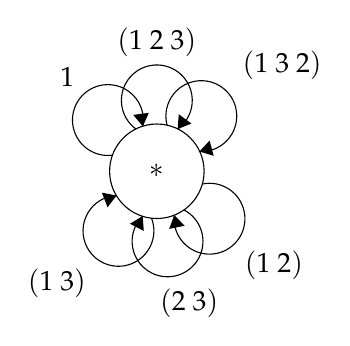
\begin{tikzpicture}[scale=0.2]
			\tikzstyle{every node}+=[inner sep=0pt]
			\draw [black] (37.4,-25.7) circle (3);
			\draw (37.4,-25.7) node {$\ast$};
			\draw [black] (34.593,-24.676) arc (277.6886:-10.3114:2.25);
			\draw (31.72,-20.34) node [above] {$1$};
			\fill [black] (36.51,-22.85) -- (36.89,-21.99) -- (35.9,-22.12);
			\draw [black] (40.276,-26.512) arc (101.97044:-186.02956:2.25);
			\draw (42.95,-31.68) node [right] {$(1\ 2)$};
			\fill [black] (38.51,-28.48) -- (38.18,-29.36) -- (39.16,-29.16);
			\draw [black] (39.111,-28.15) arc (62.6723:-225.3277:2.25);
			\draw (39.45,-33.13) node [below] {$(2\ 3)$};
			\fill [black] (36.5,-28.55) -- (35.69,-29.03) -- (36.57,-29.49);
			\draw [black] (37.059,-28.669) arc (21.17668:-266.82332:2.25);
			\draw (31.05,-31.87) node [below] {$(1\ 3)$};
			\fill [black] (34.84,-27.24) -- (33.91,-27.06) -- (34.27,-27.99);
			\draw [black] (36.077,-23.02) arc (234:-54:2.25);
			\draw (37.4,-18.45) node [above] {$(1\ 2\ 3)$};
			\fill [black] (38.72,-23.02) -- (39.6,-22.67) -- (38.79,-22.08);
			\draw [black] (38.053,-22.784) arc (195.11223:-92.88777:2.25);
			\draw (45.36,-19.95) node [above] {$(1\ 3\ 2)$};
			\fill [black] (40.11,-24.44) -- (41.01,-24.72) -- (40.75,-23.75);
			\end{tikzpicture}
		\end{center}
		\caption*{The delooping of the symmetric group $S_3$, aka $\mathbf{B}S_3$.}
	\end{figure}
	
	 The natural numbers can also be endowed with the monoid structure of addition, thus a particular instance of a single object category is the delooping of $(\N, +)$. Notice that this category is very different from the posetal category $(\N, \leq)$. In the former, $\N$ is in correspondence with the morphisms while in the latter, it is in correspondence with the objects. 
\end{exmp}
A lot of simple examples of large categories arise as subcategories of \textbf{Set}.
\begin{defn}[Subcategory]
	Let $\mathbf{C}$ be a category, a category $\mathbf{C}'$ is a \textbf{subcategory} of $\mathbf{C}$ if, the following properties are satisfied.
	\begin{enumerate}
		\item The objects and morphisms of $\mathbf{C}'$ are objects and morphisms of $\mathbf{C}$ (i.e.: $\mathbf{C}'_0 \subseteq \mathbf{C}_0$ and $\mathbf{C}'_1 \subseteq \mathbf{C}_1$).
		\item The source and target maps of $\mathbf{C}'$ are the restrictions of the source and target maps of $\mathbf{C}$ on $\mathbf{C}'_1$ and for every morphism $f \in \mathbf{C}'_1$, $s(f), t(f) \in \mathbf{C}'_0$.
		\item The composition map of $\mathbf{C}'$ is the restriction of the composition map of $\mathbf{C}$ on $\mathbf{C}'_2$ and for any $(f,g) \in \mathbf{C}'_2$, $f\circ_{\mathbf{C}'} g = f \circ_{\mathbf{C}} g \in \mathbf{C}'_1$. 
	\end{enumerate}
	Intuitively, one can see $\mathbf{C}'$ as being obtained from $\mathbf{C}$ by removing some objects and arrows, but making sure that no arrow is left with no source or no target and that no path is left without its composition. A formal consequence of 3 is that the identity morphisms of objects in $\mathbf{C}'_0$ are the same whether they are seen in $\mathbf{C}$ or $\mathbf{C}'$ (i.e.: $u_{\mathbf{C}}(A) = u_{\mathbf{C}'}(A)$ when $A \in \mathbf{C}'_0$).
\end{defn}
\begin{defn}[Full and wide]
	A subcategory $\mathbf{C}'$ of $\mathbf{C}$ is called \textbf{full} if for any objects $A,B \in \mathbf{C}'_0$, $\Hom_{\mathbf{C}'}(A,B) = \Hom_{\mathbf{C}}(A,B)$. It is called \textbf{wide} if $\mathbf{C}'_0 = \mathbf{C}_0$.
\end{defn}
\begin{exmps}[Subcategories of \textbf{Set}]\label{exmp-subcatSet}
	One can view most of the theory studied in the first year of a typical mathematics curriculum through the lens of category theory as witnessed by the following list.
	\begin{enumerate}
		\item Since the composition of injective functions is again injective, the restriction of morphisms to injective functions yields a wide subcategory of \textbf{Set}, denoted \textbf{SetInj}. Unsurprisingly, \textbf{SetSurj} can be constructed similarly.
		\item The subcategory of finite sets is denoted \textbf{FinSet}.
		\item The category of groups (resp. rings or fields) where the morphisms are group (resp. ring or field) homomorphisms is denoted \textbf{Grp}/\textbf{Ring}/\textbf{Field}.
		\item Let $k$ be a fixed field, the category of vector spaces over $k$ where the morphisms are linear maps is denoted $\textbf{Vec}_k$. The subcategory of $\textbf{Vec}_k$ consisting only of finite dimensional vector spaces is denoted $\textbf{FinVec}_k$.
		\item The category of partially ordered sets where morphisms are order-preserving functions is denoted \textbf{Poset}.
		\item The category of topological spaces where morphisms are continuous functions is denoted \textbf{Top}.
	\end{enumerate}
	All of these are examples of \textbf{concrete} categories, which, informally, are categories of sets with extra structure.
\end{exmps}

Our last example is a large category which is not a subcategory of \textbf{Set}.
\begin{exmp}[\textbf{Rel}]
    The category of sets and relations, denoted \textbf{Rel}, has as objects the collection of all sets and for any sets $X$ and $Y$, $\Hom_{\textbf{Rel}}(X,Y)$ is the set of relations between $X$ and $Y$, that is, subsets of $X\times Y$. The composition of two relations $R \subseteq X\times Y$ and $S \subseteq Y\times Z$ is defined by
    \[S\circ R = R;S := \{(x,z) \in X\times Z \mid \exists y \in Y, (x,y) \in R, (y,z) \in S\} \subseteq X \times Z.\]
    It is easy to check that this composition is associative and that, for any set $X$, the diagonal relation $\Delta_X = \{(x,x) : x \in X\} \subseteq X \times X$ is the identity relation.
\end{exmp}

\section{Functors}
The above list is far from exhaustive; there are many more mathematical objects that can fit in a category and this is a main reason for studying this subject. Indeed, categories encapsulate a natural structure that accurately represents the heart of several mathematical theories from a global and abstract perspective. Still, a category is almost never studied on its own since the abstraction it provides can make the properties of its objects more obscure. For instance, the definition of subgroups in the framework of \textbf{Grp} is quite more involved than the usual one. However, we will probably see in later classes that some surprising links can arise between seemingly unrelated subjects (e.g.: Stone duality) through the study of how different categories relate. The central tool for exhibiting these relations is a functor.

As we will show, a functor is a morphism of categories, thus, to motivate the definition, we can look at other morphisms we have encountered. A clear similarity between categories like \textbf{Set}, \textbf{Grp}, \textbf{Ring} or \textbf{Top} is that all the objects have some sort of structure that the morphisms preserve. Thus, we want to define a morphism that preserves the structure of a category which is given by the source and target maps, the composition and the identities.
\begin{defn}[Functor]
	Let $\mathbf{C}$ and $\mathbf{D}$ be categories, a \textbf{functor} $F: \mathbf{C} \rightsquigarrow \mathbf{D}$ is a pair of maps $F_0:\mathbf{C}_0 \rightarrow \mathbf{D}_0$ and $F_1:\mathbf{C}_1 \rightarrow \mathbf{D}_1$ such that diagrams \eqref{diag-func1}, \eqref{diag-func2} and \eqref{diag-func3} commute (where $F_2$ is induced by the definition of $F_1$ with $(f,g) \mapsto (F_1(f), F_1(g))$).
	
	\begin{minipage}{0.37\textwidth}
		\begin{equation}\label{diag-func1}
		\begin{tikzcd}
			\mathbf{C}_0 \arrow[d, "F_0"'] & \mathbf{C}_1 \arrow[d, "F_1"] \arrow[l, "s"'] \arrow[r, "t"] & \mathbf{C}_0 \arrow[d, "F_0"] \\
			\mathbf{D}_0 & \mathbf{D}_1 \arrow[l, "s"] \arrow[r, "t"'] & \mathbf{D}_0
		\end{tikzcd}
		\end{equation}
	\end{minipage}	
	\begin{minipage}{0.26\textwidth}
		\begin{equation}\label{diag-func2}
		\begin{tikzcd}
			\mathbf{C}_2 \arrow[d, "\circ_\mathbf{C}"'] \arrow[r, "F_2"] & \mathbf{D}_2 \arrow[d, "\circ_\mathbf{D}"] \\
			\mathbf{C}_1 \arrow[r, "F_1"'] & \mathbf{D}_1
		\end{tikzcd}
		\end{equation}
	\end{minipage}
	\begin{minipage}{0.26\textwidth}
			\begin{equation}\label{diag-func3}
		\begin{tikzcd}
			\mathbf{C}_0 \arrow[d, "u_{\mathbf{C}}"'] \arrow[r, "F_0"] & \mathbf{D}_0 \arrow[d, "u_{\mathbf{D}}"] \\
			\mathbf{C}_1 \arrow[r, "F_1"'] & \mathbf{D}_1
		\end{tikzcd}
		\end{equation}
	\end{minipage}
\end{defn}
\begin{rem}[Digesting diagrams]
	Commutative diagrams will be heavily employed to make clearer and more compact arguments (especially on the board). However, it is an acquired skill to quickly grasp their meaning and make effective use of their advantages. Unpacking the above definition will help to understand it as well as getting better with manipulating diagrams.
	
	A functor $F:\mathbf{C}\rightsquigarrow \mathbf{D}$ must satisfy the following properties.
	\begin{enumerate}[i.]
		\item For any $A, B \in \mathbf{C}_0$ and $f \in \Hom_{\mathbf{C}}(A,B)$, $F(f) \in \Hom_{\mathbf{D}}(F(A), F(B))$.
		\item If $f,g \in \mathbf{C}_1$ are composable, then $F(f\circ g) = F(f) \circ F(g)$.
		\item If $A \in \mathbf{C}_0$, then $u_{\mathbf{D}}(F(A)) = F(u_{\mathbf{C}}(A))$ (alternatively, $\id_{F(A)} = F(\id_A)$).
	\end{enumerate}
	The subscript on $F$ is omitted, as is common in the literature, because it is always clear whether $F$ is applied to an object or a morphism.
\end{rem}
\begin{exmps}[Boring examples]
	As usual, a few trivial constructions arise.
	\begin{enumerate}
		\item For any category $\mathbf{C}$, the \textbf{identity functor} $\id_{\mathbf{C}}: \mathbf{C}\rightsquigarrow \mathbf{C}$ is defined by letting $(\id_{\mathbf{C}})_0$ and $(\id_{\mathbf{C}})_1$ be identity maps on $\mathbf{C}_0$ and $\mathbf{C}_1$ respectively.
		\item Let $\mathbf{C}$ be a category and $\mathbf{C}'$ a subcategory of $\mathbf{C}$, the \textbf{inclusion functor} $I: \mathbf{C}' \rightsquigarrow \mathbf{C}$ is defined by letting $I_0$ be the inclusion map $\mathbf{C}'_0 \hookrightarrow \mathbf{C}_0$ and $I_1$ be the inclusion map $\mathbf{C}'_1 \hookrightarrow \mathbf{C}_1$.
		\item Let $\mathbf{C}$ and $\mathbf{D}$ be categories and $X$ be an object in $\mathbf{D}$, the \textbf{constant functor} $X: \mathbf{C} \rightsquigarrow \mathbf{D}$ is defined by letting $X_0(A) = X$ for any $A \in \mathbf{C}_0$ and $X_1(f) = \id_X$ for any $f \in \mathbf{C}_1$.
	\end{enumerate}
\end{exmps}
\begin{exmps}[Less boring]\label{exmp-simplediagrams}
    Functors with the domain being one of $\mathbf{1}$, $\mathbf{2}$ or $\mathbf{2}\times \mathbf{2}$ (cf. Example \ref{exmp-simplecats}) are a bit less boring. Let the codomain be a category $\mathbf{C}$ and let us analyze these functors.
    \begin{itemize}
        \item[-] Let $F: \mathbf{1} \rightsquigarrow \mathbf{C}$, $F_0$ assigns to the single object in $\bullet \in \mathbf{1}_0$ an object $F(\bullet) \in \mathbf{C}_0$. Then, by commutativity of \eqref{diag-func3}, $F_1$ is completely determined by $\id_{\bullet} \mapsto \id_{F(\bullet)}$. We conclude that functors of this type are in correspondence with objects of $\mathbf{C}$.
        
        \item[-] Let $F: \mathbf{2} \rightsquigarrow \mathbf{C}$, $F_0$ assigns to $A$ and $B$, two objects $FA, FB \in\mathbf{C}_0$ and $F_1$'s action on identities is fixed. Still, there is one choice to make for $F_1(f)$ which must be a morphism in $\Hom_{\mathbf{C}}(FA, FB)$. Therefore, $F$ sums up to a choice of two objects in $\mathbf{C}$ and a morphism between them. In other words, functors of this type are in correspondence with morphisms in $\mathbf{C}$.
        
        \item[-] Similarly (we leave the details as an exercise), functors of type $F: \mathbf{2}\times \mathbf{2} \rightsquigarrow \mathbf{C}$ are in correspondence with commutative squares inside the category $\mathbf{C}$, that is, pairs of pairs of composable morphisms $((f,g), (f',g'))$ satisfying $f \circ g = f' \circ g'$.
    \end{itemize}
\end{exmps}
\begin{rem}[Functoriality]
	We will use the term \textbf{functorial} as an adjective to qualify transformations that behave like functors and \textbf{functorality} to refer to the property of behaving like a functor.
\end{rem}
Throughout this seminar, the goal will essentially be to grow this list with more and more interesting functors and perhaps exploit their behavior wisely. Before pursuing this objective, we give important definitions analogous to injectivity and surjectivity of functions.
\begin{defn}[Full and faithful]
	Let $F:\mathbf{C} \rightsquigarrow \mathbf{D}$ be a functor. For $A,B \in \mathbf{C}_0$, denote the restriction of $F_1$ to $\Hom_{\mathbf{C}}(A,B)$ with \[F_{A,B}:\Hom_{\mathbf{C}}(A,B) \rightarrow \Hom_{\mathbf{D}}(F(A), F(B)).\]
	\begin{itemize}
		\item If $F_{A,B}$ is injective for any $A,B \in \mathbf{C}_0$, then $F$ is \textbf{faithful}.
		\item If $F_{A,B}$ is surjective for any $A,B \in \mathbf{C}_0$, then $F$ is \textbf{full}.
		\item If $F_{A,B}$ is bijective for any $A,B \in \mathbf{C}_0$, then $F$ is \textbf{fully faithful}.
	\end{itemize}    
\end{defn}
\begin{rem} 
These notions never mention the action of $F$ on objects, so they cannot lead to a notion of \textbf{isomorphism} of categories.
\end{rem}

\begin{exmps}
	For the following examples, we leave to the reader the easy and irrelevant to category theory task of proving they are actually functors.
	\begin{enumerate}
		\item The power set functor $\mP: \textbf{Set} \rightsquigarrow \textbf{Set}$ sends a set $X$ to its power set $\mP(X)$ and a function $f: X\rightarrow Y$ to the image map $\mP(f):\mP(X)\rightarrow \mP(Y)$, the latter sends a subset $S\subseteq X$ to \[f(S) = \{f(s) \mid s \in S\} \subseteq Y.\]
		The power set functor is faithful because the same image map cannot arise from two different functions, it is not full because lots of functions $\mP(X) \rightarrow \mP(Y)$ are not image maps. One can also argue by cardinality because (when $|X|, |Y| \geq 2$)
		\[|\Hom_{\textbf{Set}}(X,Y)| = |Y|^{|X|} < |\mP(Y)|^{|\mP(X)|} = |\Hom_{\textbf{Set}}(\mP(X), \mP(Y))|.\]
		\item While in general the inclusion functor of a subcategory is not interesting, there are some distinguished cases. For instance, when considering subcategories of \textbf{Set} such as those mentioned in Example \ref{exmp-subcatSet}, this functor gets a fancier denomination, namely, the \textbf{forgetful} functor (denoted $U$). This is because, morally, the functor is forgetting about the inner structure of the objects and morphisms and it outputs the underlying sets and functions.
		
		\item It is also sometimes useful to consider \textit{intermediate} forgetful functors. For instance, $U: \textbf{Ring} \rightsquigarrow \textbf{Ab}$ sends a ring $(R, +, \cdot)$ to the abelian group $(R, +)$. It acts trivially on morphisms because part of the requirements for ring homomorphisms is to preserve the underlying additive group structure.
		
		\item In some cases, there is a canonical way to go in the opposite direction of the forgetful functor, that is, the \textbf{free} functor. For \textbf{Grp}, the free functor $F: \textbf{Set} \rightsquigarrow \textbf{Grp}$ sends a set to the free group generated by this set and a function $f: X\rightarrow Y$ to the unique group homomorphism $F(X) \rightarrow F(Y)$ that restricts to $f$ on the set of generators.
		
		Later in the notes, when covering adjunctions, we will study a strong relation between the forgetful functor $U$ and the free functor $F$ that will generalize to other mathematical structures.
		
		\item Let $(X, \leq)$ and $(Y, \subseteq)$ be posets, and $F:X\rightsquigarrow Y$ be a functor between their posetal categories. For any $a, b \in X$, if $a\leq b$, then $\Hom_X(a,b)$ contains a single element, thus $\Hom_Y(F(a), F(b))$ must contain a morphism as well, or equivalently $F(a) \subseteq F(b)$. In other words, $F$ is an order-preserving function on the objects.
		
		Conversely, any order-preserving functions between $X$ and $Y$ will correspond to a unique functor since there is only one morphism in all the Hom-sets.
				
		\item Let $G$ and $H$ be groups and $\mathbf{B}G$ and $\mathbf{B}H$ be their respective deloopings, then the functors $F: \mathbf{B}G \rightsquigarrow \mathbf{B}H$ are exactly the group homomorphisms from $G$ to $H$.
		
		\item For any group $G$, the functors $F:\mathbf{B}G \rightsquigarrow \textbf{Set}$ are in correspondence with left actions of $G$. Indeed, if $S = F(\ast)$, then \[F_1: G = \Hom_{\mathbf{B}G}(\ast, \ast) \rightarrow \Hom_{\textbf{Set}}(S, S)\]
		is such that $F(gh) = F(g) \circ F(h)$ for any $g,h \in G$ and $F(1) = \id_S$. Moreover, since for any $g \in G$,
		\[\id_S = F(1) = F(gg^{-1}) = F(g) \circ F(g^{-1}),\]
		the function $F(g)$ is a bijection and we conclude $F_1$ is the permutation representation of the group action. That is, $F$ corresponds to the group action defined by $g \cdot s = F(g)(s)$ for all $g \in G$ and $s \in S$.
		
		\item In the previous example, replacing \textbf{Set} with $\textbf{Vec}_k$, one obtains $k$-linear representations of $G$ instead of actions of $G$. 
	\end{enumerate}
\end{exmps}
\begin{rem}
    From this long (and yet hardly exhaustive) list, one might get the feeling that everything is a functor. While the latter are ubiquitous in mathematics (that is one reason we study category theory), functoriality can fail for some mathematical transformations.
    
    For instance, let us define $F: \textbf{FinVec}_k \rightsquigarrow \textbf{Set}$ which assigns to any vector space over $k$ a choice of basis. There is no non-trivializing way to define an action of $F$ on linear maps which make $F$ into a functor. Another example of a non-functor is given by the center of a group in $\textbf{Grp}$: a morphism of group $H \to G$ does not necessarily send the center of $H$ in the center of $G$ (take for instance $\mathfrak{S}_2 \hookrightarrow \mathfrak{S}_3$).
\end{rem}
%TODO: Functoriality is useful to prove stuff. If you know about the fundamental group. One can show brouwer fixed point theorem using this.


In this lecture, we introduced a novel structure, namely categories, that functors preserve. Hence it is reasonable to wonder if categories are also part of a category. In fact, the only missing ingredient is the composition of functors (we already know what the source and target of a functor is and every category has an identity functor). After proving the following proposition, we end up with the category \textbf{Cat} where objects are categories and morphisms are functors. In order to avoid paradoxes of the Russel kind, it is essential to restrict \textbf{Cat} to contain only \textit{small categories}.
\begin{prop}
	Let $F:\mathbf{C}\rightsquigarrow \mathbf{D}$ and $G: \mathbf{D}\rightsquigarrow \mathbf{E}$ be functors and $G \circ F:\mathbf{C} \rightsquigarrow \mathbf{E}$ be their composition defined (naturally) by $G_0 \circ F_0$ on objects and $G_1 \circ F_1$ on morphisms. Then, $G \circ F$ is a functor.
\end{prop}
\begin{proof}
	One could proceed with a really \textit{hands-on} proof and show that $G \circ F$ satisfies the three necessary properties in a straightforward manner. While this should not be too hard, the proof will end up involving objects, morphisms and the composition from all three different categories. This can easily lead to confusion or worse, boredom!
	
	Instead, we will use the diagrams we introduced in the first definition of a functor. From the functoriality of $F$ and $G$, we get two sets of three diagrams and combining them yields the diagrams for $G \circ F$.
	
	\begin{equation}\label{diag-comp1}
		\begin{tikzcd}
			\mathbf{C}_0 \arrow[d, "F_0"'] & \mathbf{C}_1 \arrow[d, "F_1"] \arrow[r, "t"] \arrow[l, "s"'] & \mathbf{C}_0 \arrow[d, "F_0"] \\
			\mathbf{D}_0 \arrow[d, "G_0"'] & \mathbf{D}_1 \arrow[d, "G_1"] \arrow[r, "t"] \arrow[l, "s"'] & \mathbf{D}_0 \arrow[d, "G_0"] \\
			\mathbf{E}_0                   & \mathbf{E}_1 \arrow[r, "t"] \arrow[l, "s"']                  & \mathbf{E}_0                 
		\end{tikzcd}
	\end{equation}
	\begin{minipage}{0.48\textwidth}
		\begin{equation}\label{diag-comp2}
			\begin{tikzcd}
				\mathbf{C}_2 \arrow[r, "F_2"] \arrow[d, "\circ_{\mathbf{C}}"'] & \mathbf{D}_2 \arrow[r, "G_2"] \arrow[d, "\circ_{\mathbf{D}}"] & \mathbf{E}_2 \arrow[d, "\circ_{\mathbf{E}}"] \\
				\mathbf{C}_1 \arrow[r, "F_1"']                      & \mathbf{D}_1 \arrow[r, "G_1"']                     & \mathbf{E}_1                     
			\end{tikzcd}
		\end{equation}
	\end{minipage}
	\begin{minipage}{0.48\textwidth}
			\begin{equation}\label{diag-comp3}
				\begin{tikzcd}
					\mathbf{C}_0 \arrow[r, "F_0"] \arrow[d, "u_{\mathbf{C}}"'] & \mathbf{D}_0 \arrow[r, "G_0"] \arrow[d, "u_{\mathbf{D}}"] & \mathbf{E}_0 \arrow[d, "u_{\mathbf{E}}"] \\
					\mathbf{C}_1 \arrow[r, "F_1"']                  & \mathbf{D}_1 \arrow[r, "G_1"']                 & \mathbf{E}_1                 
				\end{tikzcd}
		\end{equation}
	\end{minipage}\\
	Almost no argument is needed here as the commutativity of the smaller diagrams clearly implies the commutativity of the combined diagrams. One information that is not shown above is the fact that $(G\circ F)_2 = G_2 \circ F_2$, but it would be pedantic to prove this.
\end{proof}
Since functors are also a new structure, one might expect that there are transformations between functors that preserve it. It is indeed the case, they are called \textbf{natural transformations} and they are the main subject of Lecture 5. Moreover, although we might not cover it, there is a whole tower of abstraction that one could build in this way and it is the subject of study of higher category theory.

\end{document}

